%Photoshop techniques for changing skintone from select online video tutorials
\subsection{Changing skin colour from dark to light \cite{photoshop:obama}}\label{app:photoshop_obama}

\subsubsection*{Effect}
\begin{longtable}{|c|c|}
    \caption{Screen captures from Photoshop tutorial for changing skin colour from dark to light.}\\
    \hline
    Original & Result \\
    \hline
  \begin{minipage}{.29\textwidth}
    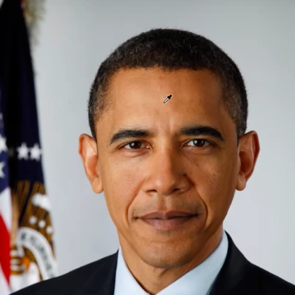
\includegraphics[width=\textwidth,height=\textheight,keepaspectratio]{images/obama_orig}
  \end{minipage} & 
  \begin{minipage}{.29\textwidth}
    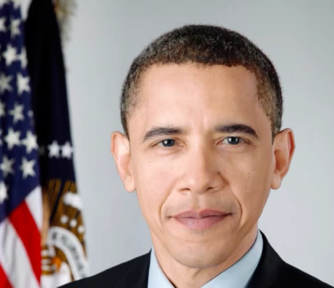
\includegraphics[width=\textwidth,height=\textheight,keepaspectratio]{images/obama_res}
  \end{minipage} \\
    \hline
\end{longtable}

\subsubsection*{Summary of the process}
\begin{itemize}
  \item Levels adjustment layer - Make gamma value adjustment, adjusting midtones, and adjust the white point for overall brightening effect
  \item Curves adjustment layer - Reduce highlights resulting from brightening with a custom curve dipping at the highlights
  \item HSV adjustment layer - Reduce saturation, correcting the oversaturation caused by brightening the image
  \item Further brightening: obtain greyscale image; boost reds and yellows in the greyscale conversion, brightening the skin area, then use greyscale image to inform the original image’s luminosity; set this effect to a reduced opacity for a more natural appearance
  \item Adjust colours by eye with a colour balance layer 
\end{itemize}
\pagebreak

\subsection{Matching the skintones of face and body \cite{photoshop:match_body}}\label{app:photoshop_match_body}

\subsubsection*{Effect}
\begin{longtable}{|c|c|c|}
    \caption{Screen captures from Photoshop tutorial for matching the skintones of face and body.}\\
    \hline
    Original & Target & Result \\
    \hline
  \begin{minipage}{.29\textwidth}
    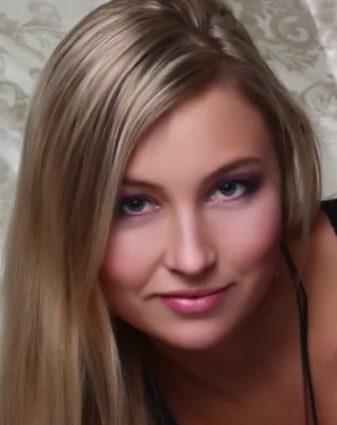
\includegraphics[width=\textwidth,height=\textheight,keepaspectratio]{images/match_body_orig}
  \end{minipage} & 
  \begin{minipage}{.29\textwidth}
    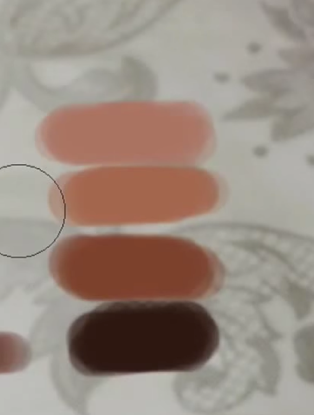
\includegraphics[width=\textwidth,height=\textheight,keepaspectratio]{images/match_body_targ}
  \end{minipage} & 
  \begin{minipage}{.29\textwidth}
    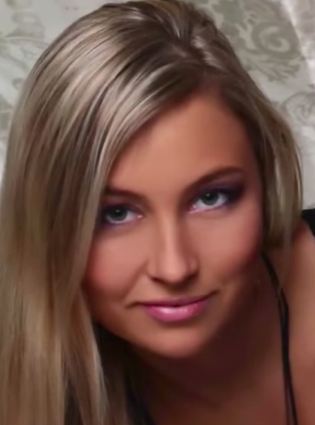
\includegraphics[width=\textwidth,height=\textheight,keepaspectratio]{images/match_body_res}
  \end{minipage} \\
    \hline
\end{longtable}

\subsubsection*{Summary of the process}
\begin{itemize}
  \item Sample a range of colours from face and body (the area with the desired colour) and determine by eye if face should become warmer or cooler, or lighter or darker
  \item Simultaneously adjust brightness and colour with levels adjustment for each colour channel, adjusting the output and input white and black points
    \begin{itemize}
      \item For darker and warmer colours, add yellow and magenta to the image highlights while simultaneously dimming the image by lowering the output white points
    \end{itemize}
  \item Reduce saturation to counteract oversaturation caused by colour adjustment
  \item Reduce opacity of effect for more natural appearance
\end{itemize}
\pagebreak

\subsection{Matching the skintones of portraits of different people \cite{photoshop:match_other} }\label{app:photoshop_match_other}

\subsubsection*{Effect}
\begin{longtable}{|N||c|c|c|}
    \caption{Screen captures from Photoshop tutorial for matching the skintones of portraits of different people.}\\
    \hline
    \multicolumn{1}{|c||}{No.} & Original & Target & Result \\
    \hline  \label{row:photoshop_match_other_1} &
  \begin{minipage}{.29\textwidth}
    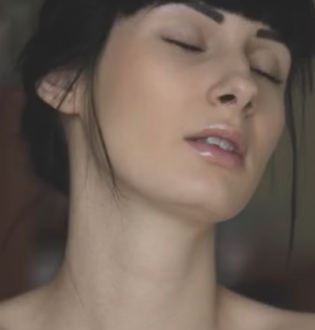
\includegraphics[width=\textwidth,height=\textheight,keepaspectratio]{images/match_other_1_orig}
  \end{minipage} & 
  \begin{minipage}{.29\textwidth}
    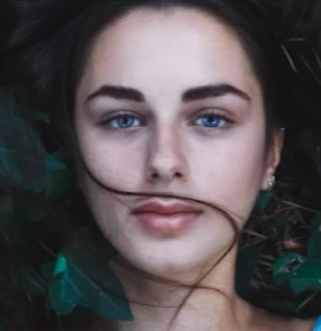
\includegraphics[width=\textwidth,height=\textheight,keepaspectratio]{images/match_other_1_targ}
  \end{minipage} & 
  \begin{minipage}{.29\textwidth}
    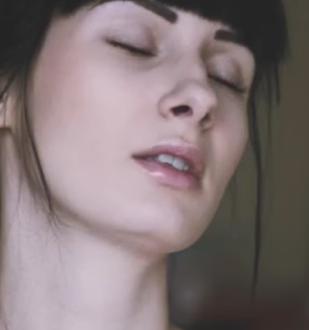
\includegraphics[width=\textwidth,height=\textheight,keepaspectratio]{images/match_other_1_res}
  \end{minipage} \\
    \hline  \label{row:photoshop_match_other_2} &
  \begin{minipage}{.29\textwidth}
    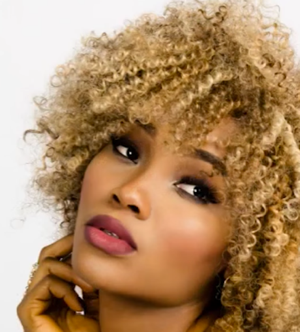
\includegraphics[width=\textwidth,height=\textheight,keepaspectratio]{images/match_other_2_orig}
  \end{minipage} & 
  \begin{minipage}{.29\textwidth}
    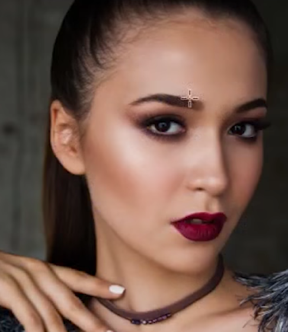
\includegraphics[width=\textwidth,height=\textheight,keepaspectratio]{images/match_other_2_targ}
  \end{minipage} & 
  \begin{minipage}{.29\textwidth}
    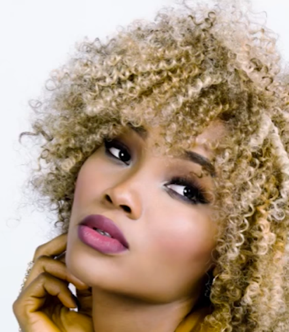
\includegraphics[width=\textwidth,height=\textheight,keepaspectratio]{images/match_other_2_res}
  \end{minipage} \\
    \hline
\end{longtable}

\subsubsection*{Summary of the process}
\begin{itemize}
  \item For both the target and original image, select an area on face with even skin tone and calculate the average colour. It is important to select the same areas on both images for the effect to work - if the cheek is selected for one person, the cheek should be selected for other person as well
  \item Using the curves adjustment layer, adjust the curves for each channel, manipulating the point of the original colour and the target colour such that the output of the original color is equal to the target colour
  \item Make some additional adjustments to the curve to change brightness and contrast
  \item Sometimes the colour curves will have to be further adjusted by eye; sometimes, different areas of the skin must be adjusted separately – what works for the face may not work for the body areas
\end{itemize}